There exist a host of alternatives to the forward and backward Euler methods
for approximating the solution of the differential equation
$\Bx'(t) = \BA\Bx(t)$.
For example, the \emph{trapezoid method} has the form
\[ \Bx_{k+1} = \Bx_k + {\textstyle{1\over2}} \Delta t \BA(\Bx_k + \Bx_{k+1}),\]
where $\Delta t >0$ is the time-step, and $\Bx_k \approx \Bx(t_k)$ for $t_k = k\Delta t$.

\begin{enumerate}
\item Like backward Euler, the trapezoid method is an \emph{implicit} technique:
      $\Bx_{k+1}$ appears on both the right and left hand side of the formula 
      above that defines it.
      Describe how to find $\Bx_{k+1}$ given $\Bx_k$.  In particular, what linear system 
      of algebraic equations needs to be solved at each step?  (For comparison, the backward 
      Euler method requires the solution of the system $(\BI-\Delta t \BA)\Bx_{k+1} = \Bx_k$
      for the unknown $\Bx_{k+1}$ at each step.)

\item Consider the matrix and initial condition
      \[ \BA = \bmatrix{-1 & 10 \cr 0 & -2}, \quad \Bx(0) = \bmatrix{1\cr 1}.\]
      Approximate the solution to $\Bx'(t) = \BA\Bx(t)$ on the interval $t\in[0,5]$
      for time step $\Delta t=.05$.
      Produce a {\tt semilogy} plot showing $t_k=k\Delta t $ versus $\norm{\Bx_k}$ 
      for $k=0, \ldots, 100$.  (Use the {\tt norm} command in MATLAB to compute $\norm{\Bx_k}$.)

% \hfill \emph{continued on the next page}      
\item We wish to understand how the error in our approximation at time $t=1$ improves as we
      run the simulation with smaller and smaller $\Delta t$ values.
      Produce a {\tt loglog} plot showing $\Delta t$ versus the error in the trapezoid rule
      and backward Euler approximations for the matrix and initial condition
      in part~(b) at time $t=1$.  To compute the error, first find the exact
      solution $\Bx(1) = \eop^{\BA} \Bx(0)$ using the {\tt expm} command, 
      then compute the norms $\norm{\widehat{\Bx}-\Bx(1)}$, 
      where $\widehat{\Bx}$ denotes your approximation
      to $\Bx(1)$ from the trapezoid or backward Euler methods. 
      Start your plot with $\Delta t=1/2$ and use sufficiently many smaller values
      of $\Delta t$ to make the trend in your plot clear.  For which method does the
      error decay more rapidly as $\Delta t \to 0$?

\vspace*{1em}
\item Forward Euler iterates can be written as $\Bx_{k} = (\BI+\Delta t \BA)^k \Bx_0$,
      while backward Euler iterates can be written as $\Bx_{k} = (\BI-\Delta t \BA)^{-k} \Bx_0$.

\vspace*{.25em}
      Work out a similar formula for the iterates $\Bx_k$ generated by the trapezoid method.

\vspace*{.25em}
      Suppose $\BA = \BV\BLambda\BV^T$ is symmetric, and all of its 
      eigenvalues $\lambda_j$, $j=1,\ldots, n$, are negative.  
      How must you choose the time step $\Delta t$ to ensure that the iterates
      $\Bx_k$ generated by the trapezoid method converge to zero, $\|\Bx_k\|\to 0$,
      as $k\to\infty$\,?
\end{enumerate}

%%%%%%%%%%%%%%%%%%%%%%%%%%%%%%%%%%%%%%%%%%%%%%%%%%%%%%%%%%%%%%%%%%%%%%%%%%%%%%%%
\ifthenelse{\boolean{showsols}}{\begin{solution}
\begin{enumerate}
\item Given the trapezoid rule
      \[ \Bx_{k+1} = \Bx_k + {\textstyle{1\over2}} \Delta t \BA(\Bx_k + \Bx_{k+1}),\]
      group all terms involving $\Bx_{k+1}$ on the left and $\Bx_k$ on the right to obtain
       \[ (\BI - {\textstyle{1\over2}} \Delta t \BA) \Bx_{k+1}  
          =  (\BI + {\textstyle{1\over2}} \Delta t \BA) \Bx_{k}.\]
      One can solve then solve this system for $\Bx_{k+1}$ (e.g., using MATLAB's `backslash' command).   
      Alternatively, invert the matrix on the left to obtain a formula for $\Bx_{k+1}$:
       \[ \Bx_{k+1} = (\BI-{\textstyle{1\over2}}\Delta t \BA)^{-1}
                      (\BI+{\textstyle{1\over2}}\Delta t \BA) \Bx_k.\]
      (Either of these forms is acceptable for full credit.)

%%%%%%%%%%%%%%%%%%%%%%%%%%%%%%%%%%%%%%%%%%%%%%%%%%%%%%%%%%%%%%%%%%%%%%%%%%%%%%%%
\item The plot below shows the growth of norm of the solution $\Bx_k$ 
      as a function of $k$ for $\Delta t = .05$.  
      Though both eigenvalues of $\BA$ are negative, there is transient
      growth in $\Bx_k$ before the eventual decay.

      \begin{center} 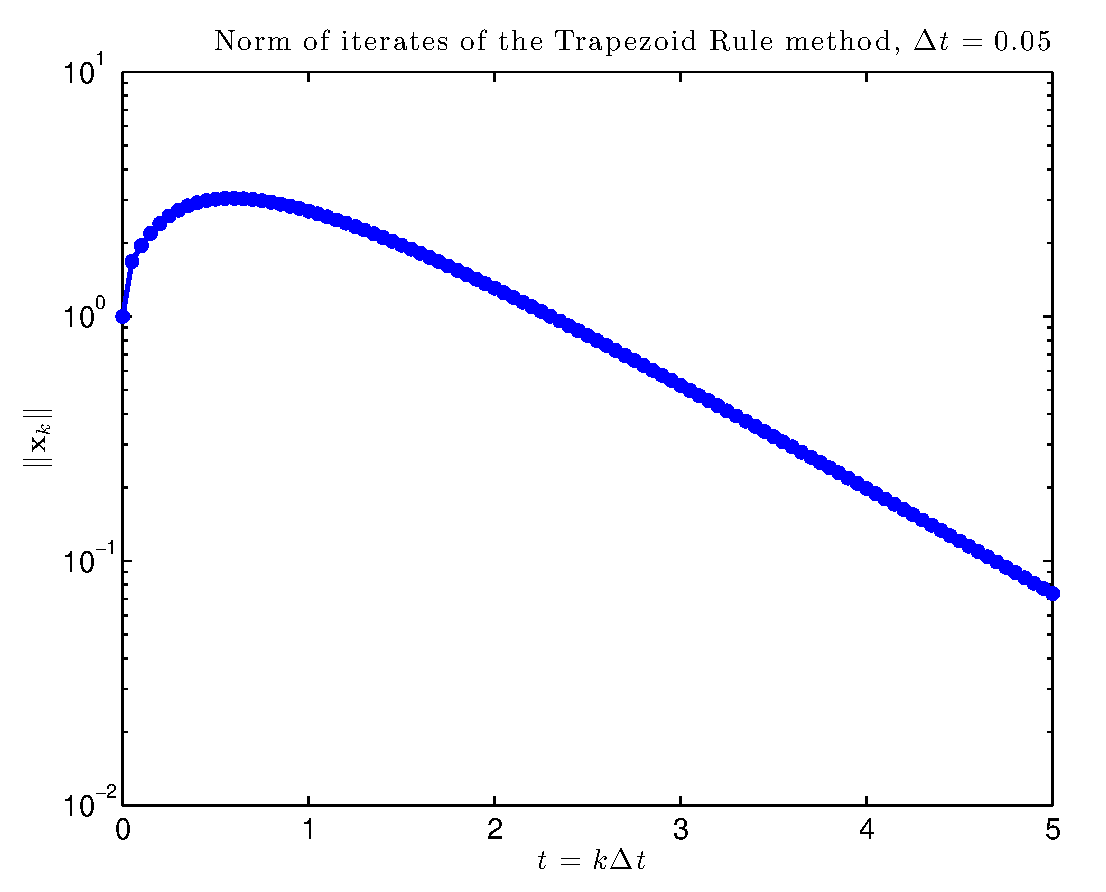
\includegraphics[scale=0.5]{traprule1}\end{center}

      \input traprule_code1

%%%%%%%%%%%%%%%%%%%%%%%%%%%%%%%%%%%%%%%%%%%%%%%%%%%%%%%%%%%%%%%%%%%%%%%%%%%%%%%%
\item The following plot shows the error in the backward Euler and trapezoid rule
      computations as a function of the step size $\Delta t$.  (Note use of the
         {\tt set('gca','Xdir','reverse')} command to reverse the direction of the
          horizontal axis so that $\Delta t$ decreases from left to right.

      [GRADERS: Please deduct 7~points if the two lines have the same slope.
      This error most likely comes from students comparing the approximate 
      solution at time $t=1\pm \Delta t$ to the true solution at $t=1$.]

      \begin{center} 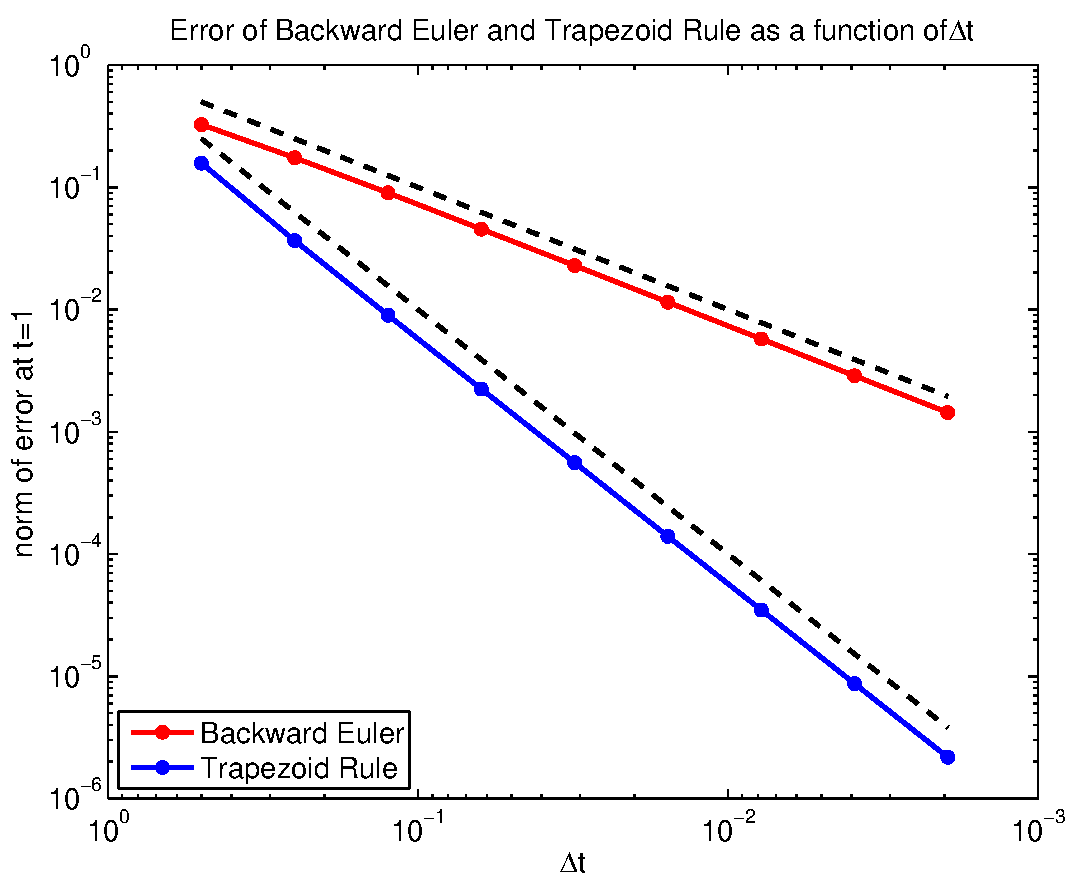
\includegraphics[scale=0.5]{traprule2}\end{center}

      The black dashed lines show $\Delta t$ and $(\Delta t)^2$:  Note that
      the backward Euler error decreases at the rate $\Delta t$, while
      the trapezoid rule decreases at the rate $(\Delta t)^2$.
      Thus, as $\Delta t$ is cut in half, the trapezoid rule error is
      quartered.  Thus, the trapezoid rule is considerably better.

      (Though not necessary for this problem, a complete analysis would
       also consider the amount of work required at each step.
       On that count the trapezoid rule is a bit more expensive,
         as it requires an extra matrix-vector multiplication at each step.)

      \input traprule_code2

%%%%%%%%%%%%%%%%%%%%%%%%%%%%%%%%%%%%%%%%%%%%%%%%%%%%%%%%%%%%%%%%%%%%%%%%%%%%%%%%
\item  The formula in part~(a) enables the computation we need to make for this part.
       First, by applying $k$ steps of the trapezoid method, we have the formula 
       \[ \Bx_k = (\BI-{\textstyle{1\over2}}\Delta t \BA)^{-k}
                      (\BI+{\textstyle{1\over2}}\Delta t \BA)^k \Bx_0.\]

       Next, the problem asks how the method will behave as $k\to\infty$ 
       if $\BA$ is symmetric with all eigenvalues negative.
       In this case write $BA = \BV\BLambda\BV^T$, so that
       \begin{eqnarray*}
         \Bx_k &=& (\BI-{\textstyle{1\over2}}\Delta t \BA)^{-k}
                      (\BI+{\textstyle{1\over2}}\Delta t \BA)^k \Bx_k \\[0.5em]
               &=& \BV (\BI-{\textstyle{1\over2}}\Delta t \BLambda)^{-k}
                      (\BI+{\textstyle{1\over2}}\Delta t \BLambda)^k \BV^T\Bx_k.
       \end{eqnarray*}
       The diagonal entries in 
        \[ (\BI-{\textstyle{1\over2}}\Delta t \BLambda)^{-k}
                      (\BI+{\textstyle{1\over2}}\Delta t \BLambda)^k\]
       have the form
       \[ {(1 + {1\over2} \Delta t \lambda)^k \over (1-{1\over2} \Delta t \lambda)^k}
         = \left({1 + {1\over2} \Delta t \lambda \over 1-{1\over2} \Delta t \lambda}\right)^k,\] 
       and so the behavior of $\Bx_k$ as $k\to\infty$ will be controlled by 
        \[ \left|{1 + {1\over2} \Delta t \lambda \over 1-{1\over2} \Delta t \lambda}\right|.\]
       If this quantity is less than one for all eigenvalues $\lambda$ of $\BA$, 
       then $\Bx_k \to \Bzero$ as $k\to\infty$.
       If any of these quantities is larger than one, there exist initial conditions for which
       $\norm{\Bx_k}\to\infty$ as $k\to\infty$.

\vspace*{1em}
       {[GRADERS: Please deduct 3 points if the student does not make the following key observation.]}

\vspace*{1em}
       We have not yet used the fact that $\lambda < 0$.  What do we learn from this?
       If $\lambda<0$, then 
       \[ |1-{1\over2} \Delta t \lambda| = 1+{1\over 2} \Delta t |\lambda| > 
       |1+{1\over 2} \Delta t \lambda|, \]
      and so
        \[ \left|{1 + {1\over2} \Delta t \lambda \over 1-{1\over2} \Delta t \lambda}\right| < 1.\]
      Hence, $\Bx_k \to \Bzero$ for all initial conditions.

\end{enumerate}
\end{solution}}{}

